\chapter{Теоретическая часть}

\section{Задача о многомерном рюкзаке}
В данной работе рассматривается задача о многомерном рюкзаке\\(Multidimensional 0-1 knapsack problem, MKP).
Эта задача является модификацией классической задачи о рюкзаке, поставленной в 19 веке Джорджем Мэттьюсоном. (см. \cite{Мэттьюс1897})
Данный же вариант задачи впервые был предложен Клиффордом Петерсеном в 1967 году.(см. \cite{Петерсен1967})
\subsection{Постановка задачи}
Постановка задачи такова:\\

%Неформальный вариант 
Пусть существует набор S, состоящий из N предметов, каждый из которых имеет стоимость $c_i\in\mathbb{R}^+$ и набор размеров S $s_{ij}\in\mathbb{R}^+$, где $i\in{1,2,...,N}$, $j\in{1,2,...,M}.$, $M,N\in\mathbb{N}$
Пусть также существует рюкзак с ограничениями по вместимости по измерениям $r_j\in\mathbb{R}^+$. 
Требуется максимизировать сумму
\[\sum_{i=1}^N{c_i x_i}\]
где $x_i\in\{0,1\}$ при условии
\begin{equation}\label{Valid}
\sum_{i=1}^N{s_{ij} x_i}< r_j
 \forall j\in\{1,2,…,M\}\
\end{equation}
Обычную задачу о рюкзаке можно рассматривать как частный случай при $M=1$.
И обычная задача, и её модификация являются NP-полными задачами. 
\subsection{Доказательство NP-полноты}
Для доказательства NP-полноты рассматриваемой задачи достаточно доказать NP-полноту обычной задачи о рюкзаке.
Сначала покажем, что задача принадлежит к классу NP. Входными данными является набор предметов S, процесс проверки правильности решения заключается в вычислении сумм \[\sum_{i\in S}{s_i x_i}\] и  \[\sum_{i\in S}{c_{i} x_i}\] Очевидно, такое вычисление требует затрат полиномиального времени в зависимости от вводимых данных.\\ 

Затем покажем что задача о рюкзаке является NP-полной. Для этого воспользуемся задачей разбиения множества чисел, для которой доказана NP-полнота. 
Требуется пооказать, что существует такая полиномиальновременная редукция $Q(\dot)$, что $Q(X)$ дает ответ <<Да>> для задачи о рюкзаке тогда, и только тогда, когда $X$ даёт ответ <<Да>> для задачи разбиения.\\
Обозначим ёмкость рюкзака как $R$, максимум, для которого рассматривается задача как $V$. 
Предположим, что существует набор $a_i$ для задачи разбиения, рассмотрим соответствующую ему задачу о рюкзаке:$c_i=a_i, s_i=a_i \forall i\in\{1,2,...,N\}$, при этом \[R=V=\frac{1}{2}\sum_{i=1}^{n}a_i\]. $Q(\dot)$ здесь - процесс, преобразующий задачу о разбиении к задаче о рюкзаке. Очевидно, что этот процесс является полиномиальным от входных данных.\\
Если $X$ является тем случаем, для которого залача о разбиении имеет ответ  <<Да>>, то существуют такие множества $S$ и $T$, что
\[\sum_{i\in S}a_i=\sum_{i\in T}a_i=\frac{1}{2}\sum_{i=1}^{n}a_i\].
Пусть наш рюкзак содержит предметы из $S$, из чего следует, что \[\sum_{i\in S}s_i=\sum_{i\in S}a_i=R\] и \[\sum_{i\in S}c_i=\sum_{i\in S}a_i=V\]. Следовательно, $Q(X)$ является случаем с ответом <<Да>> для задачи о рюкзаке.\\
Наоборот, если $Q(X)$ является случаем с ответом <<Да>> для задачи о рюкзаке, рассмотрим для выбранного набора $S$ такое $T$, что $T=\{1,2,...,n\}\sim S$. 
Имеем \[\sum_{i\in S}s_i=\sum_{i\in S}a_i\leq R=\frac{1}{2}\sum_{i=1}^{n}a_i\], 
и также \[\sum_{i\in S}c_i=\sum_{i\in S}a_i\geq V=\frac{1}{2}\sum_{i=1}^{n}a_i\]
Отсюда получаем, что \[\sum_{i\in S}a_i=\frac{1}{2}\sum_{i=1}^{n}a_i\] 
и \[\sum_{i\in T}a_i=\sum_{i=1}^{n}a_i-\frac{1}{2}\sum_{i=1}^{n}a_i=\frac{1}{2}\sum_{i=1}^{n}a_i\]
Следовательно, $\{S,T\}$ --искомое разбиение, и $X$ является случаем с ответом <<Да>> для задачи о разбиении. Таким образом, NP-полнота задачи о рюкзаке доказана.
%можно доказать


Вычислительная сложность задачи такого рода при переборном решении для N предметов - $ O(2^MN^3) $, что, вкупе с NP-сложностью, делает алгоритмическое решение такой задачи неэффективным для больших N.
Однако такие задачи могут быть решены эвристическими алгоритмами, то есть алгоритмами, для которых их корректность строго не доказана. 

\section{Генетические алгоритмы}

Генетические алгоритмы являются семейством в множестве эвристических алгоритмов. Впервые такой алгоритм был предложен А. Фразером. (см \cite{Фразер1970})
%эффективно применяются для решения одномерных рюкзаков - найти пруфы.
Алгоритм является итеративным.
Генетический алгоритм моделирует естественные процессы эволюции популяции, а именно - мутацию и скрещивание.
Решение задачи с помощью такого алгоритма требует нескольких предварительных этапов:
\begin{itemize}
	\item Выбор кодирования генотипа.\\
На этом этапе нужно выбрать способ кодирования генотипа, который будет эффективен для данной задачи. Такой генотип должен однозначно моделировать сущность, рассматриваемую в задаче.
	\item Выбор начального приближения.\\
Для запуска итерационного процесса требуется создать начальное множество - пул генотипов. В зависимости от способа задания начального пула скорость поиска оптимального решения может меняться. Размер пула также оказывает влияние на эффективность алгоритма: слишком маленький пул подавляет разнообразие и приводит к попаданию в локальные максимумы, слишком большой - увеличивает число операций на каждой итерации, чем замедляет работу алгоритма.
	\item Выбор мутации.\\
На каждой итерации алгоритма заранее определенная часть пула генотипов подвергется мутациям, то есть определенным образом изменяются их составляющие. Если мутирует слишком малая часть пула, то генетический алгоритм не сможет покинуть локальные максимумы, если же слишком большая - алгоритм потеряет свойство сохранения признаков.
	\item Выбор механизма скрещивания (кроссинговера).\\
После мутации происходит создание новых генотипов из частей старых с сохранением признаков родителя. Алгоритм скрещивания позволяет получить из двух родительских генотипов два различных дочерних генотипа.
	\item Выбор функции оценки(фитнесс-функции).\\
Такая функция позволяет оценивать генотипы с точки зрения их близости к оптимальному решению и отбирать из них лучшие на каждой итерации.
\end{itemize}

\subsection{Этапы работы алгоритма}%Тоже переделать.
\begin{itemize}%Это место стоит проверки
\item Создается пул генотипов с использованием заданного алгоритма начального приближения
\item Запускается итерационный процесс
	\subitem Случайным образом выбирается часть пула, которая подвергнется мутации
	\subitem Выбранная часть пула генотипов мутируется с использованием заданного алгоритма мутации
	\subitem Мутировавшие генотипы замещают собой исходные в пуле, немутировавшие остаются без изменений
	\subitem Из пула генотипов выбираются пары для скрещивания
	\subitem Производится скрещивание с использованием заданного алгоритма
	\subitem С использованием заданной функции оценки из результатов скрещивания выбираются лучшие 
	\subitem Если выполнено условие останова - например, достигнут предел числа итераций или известный максимум, то итерационный процесс завершается, в противном случае  начинается следующая итерация.
\item Результат итерационного процесса отдается пользователю
\end{itemize}

\subsection{Выбор этапов}%ПЕРЕДЕЛАЙ И ПРОВЕРЬ
Наиболее естественным кодированием отдельного решения задачи о рюкзаке в генотип является бинарная последовательность длины N, состоящая из нулей и единиц.
Каждый i-й элемент такой последовательности является индикатором вхождения i-го предмета в текущее решение. Такая модель требует наличия проверки корректности генотипа - соблюдения условия \ref{Valid} 
\\ Для генерации начального приближения был использован жадный алгоритм. Сначала создается генотип из единиц, соответствующий конфигурации рюкзака, в который положены все предметы. Затем в случайном порядке единицы заменяются на нули, пока полученныая конфигурация не будет удовлетворять условию коррекности. После этого полученный генотип мутируется с помощью текущей мутации до заполнения пула решений.
\\ В ходе работы было реализовано несколько алгоритмов мутации и скрещивания с целью сравнения их эффективности. Были реализованы следующие алгоритмы мутации:
\begin{itemize}
	\item Мутация в одной позциции, при которой заменяется значение в одной случайно выбранной точке генотипа(см. \ref{mutation1}).
	\item Инверсионная мутация, при которой половина генотипа заменяется на противоположные значения(см. \ref{mutation2}).
\end{itemize}
\FloatBarrier
	\begin{figure}[htbp]	
	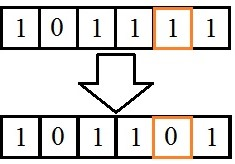
\includegraphics[width=0.3\textwidth]{./Pics/1.jpg}
	\caption{Одноточечная мутация}
	\label{mutation1}
	\end{figure}	

	\begin{figure}[htbp]
	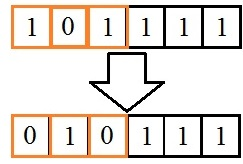
\includegraphics[width=0.3\textwidth]{./Pics/2.jpg}
		\caption{Инверсионная мутация}
	\label{mutation2}
	\end{figure}	
\FloatBarrier
 Были реализованы следующие алгоритмы скрещивания:
 \begin{itemize}
	\item Скрещивание по одной точке, при котором выбирается произвольная точка в последовательнсти генотипа, значения до точки берутся от первого генотипа, после - от второго(см. \ref{crossing1}). 
	\item Скрещивание по двум точкам, при котором выбираются две различные произвльные точки, значения внутри интервала и в самих точках берутся из первого генотипа, вне интервала - из второго(см. \ref{crossing2}). 
	\item Побитовое скрещивание, при котором значения на нечетных позициях берутся из первого генотипа, на четных - из второго(см. \ref{crossing3}).  
 \end{itemize}
\FloatBarrier
	\begin{figure}[htbp]
	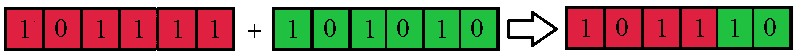
\includegraphics[width=0.7\textwidth]{./Pics/3.jpg}
	\caption{Скрещивание по одной точке}
	\label{crossing1}
\end{figure}

	\begin{figure}[htbp]
	
\includegraphics[width=0.7\textwidth]{./Pics/4.jpg}
	\caption{Скрещивание по двум точкам}
	\label{crossing2}
\end{figure}

	\begin{figure}[htbp]
	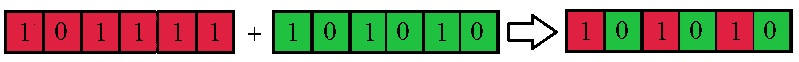
\includegraphics[width=0.7\textwidth]{./Pics/5.jpg}
	\caption{Побитовое скрещивание}
	\label{crossing3}
\end{figure}
\FloatBarrier
 В качестве функции оценки используется стоимость всех предметов, содеражщихся в рюкзаке, соответствующем конфигурации.
 
\subsection{Дополнения алгоритма}
В связи со спецификой задачи в алгоритм были внесены дополнения. 
\\Были введены проверки генотипов на корректность после мутации и скрещивания Если генотип не удовлетворяет условию корректности, то значения начиная с первой позиции начинают зануляться до достижения генотипом корректности. 
\\Были введены дополнительные пулы лучших конфигураций за время работы алгоритма. Такие пулы решают одновременно несколько задач 
\begin{itemize}
 \item Недопущение сильного ухудшения результатов решения вследствие случайных мутаций. При достаточно сильном ухудшении средней стоимости пула текущий пуз замещается текущим пулом лучших конфигураций 
 \item Возможность сохранения результатов при перезапуске алгоритма с другим начальным приближением. Такой перезапуск оправдан при получении генотипа - локального максимума, покинуть который с помощью мутации невозможно. Перезапуск алгоритма происходит при продолжительном сохранении лучшего значения в пуле конфигураций неизменным.
 \item Возможность сравнения решений после окончания работы алгоритма
\end{itemize}